\chapter{Análisis de las correlaciones entre las distintas métricas}
\addcontentsline{toc}{chapter}{Análisis de las correlaciones entre las distintas métricas}

En primer, las correlaciones que más nos interesan son las de las distintas métricas con la variable \emph{Grade}. En la Figura \ref{fig:correlations} podemos ver que no todas las métricas correlan con la misma.

\begin{figure}[H]
    \centering
    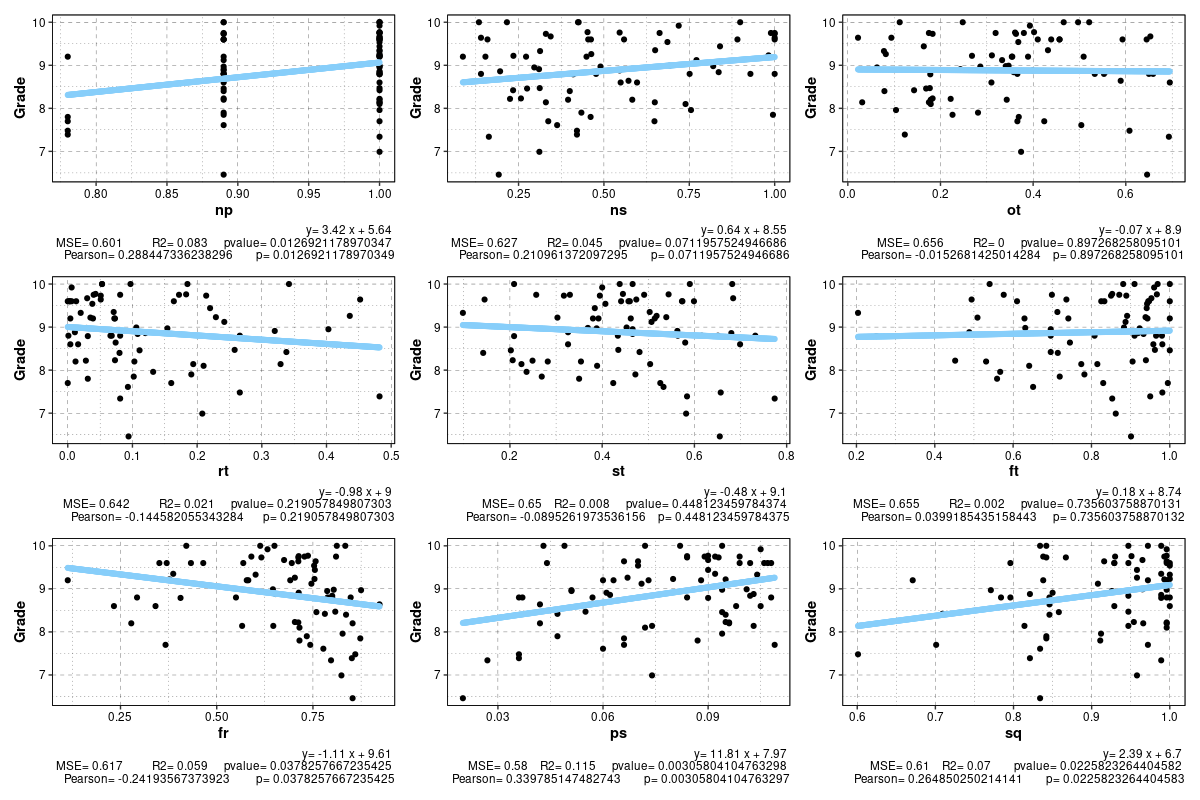
\includegraphics[width=\textwidth]{correlations.png}
    \caption{Correlaciones existentes entre las distintas métricas y la variable \emph{Grade}.}
    \label{fig:correlations}
\end{figure}

Así pues, vemos que las variables \emph{np} ($p = 0.0127 < 0.05$), \emph{fr} ($p = 0.0378 < 0.05$),    \emph{ps} ($p = 0.0031 < 0.05$) y \emph{sq} ($p = 0.0226 < 0.05$) correlan con la calificación obtenida y que la variable \emph{ns} podría correlar con la variable \emph{Grade} aunque con un grado de certeza menor que el resto ($p = 0.0712 < 0.1$).